\section{Evaluation}\label{evaluation}
In this section, we evaluate the performance overhead due to the control mechanism we have implemented in android kernel. In our experimental set up, we use original  and modified Goldfish Kernel on a emulator on a Linux machine for testing. 

\subsection{Experimental Goal}
Our idea focuses on  giving the control to  user on how the energy will be spent by different apps installed on the mobile phone. So, it becomes equally important to check and make sure that user does not see major performance hit in the system while using. So, the end goal of this  experiment is to obtain performance overhead in terms of time introduced due to our changes and finally conclude that it is remains almost constant in different scenarios and within order of few milliseconds or seconds so that quality of user experienced is not compromised.


\subsection{Methodology}
\begin{figure}[t]
	%\vspace{0.2in}
	\centering
	%\resizebox{0.7\linewidth}{!}{
	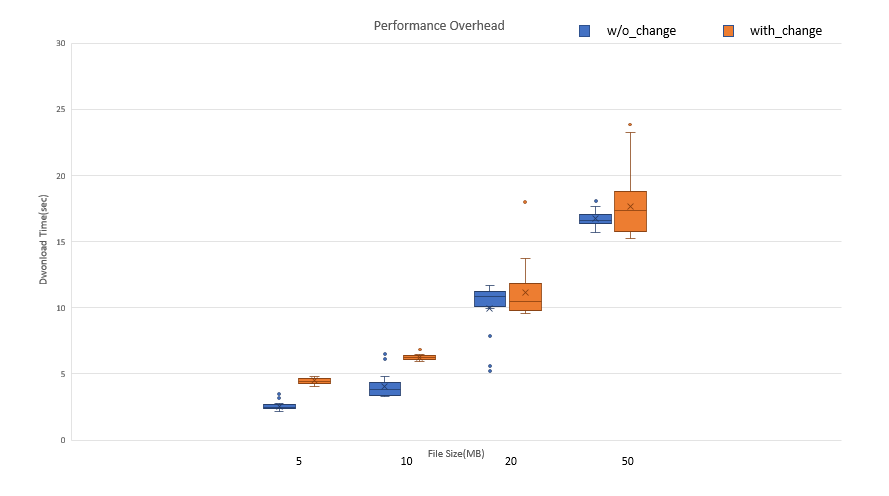
\includegraphics[width=\linewidth]{Figs/boxplot}
	%}
	\caption{Results for file downloads}
	\label{fig:result}
	\centering
\end{figure}

We developed a simple android app using which a user has options to download files of different sizes. In our experiment, we download a file of size 5 MB 20 times from server[https://www.thinkbroadband.com/download]and this is  repeated for files of other sizes i.e. 10MB, 20MB, 50MB one after another from same server using our custom android app on the Android emulator. This experiment is conducted for two cases when (i) Emulator is running original/unmodified Goldfish kernel  (ii) Emulator is running Goldfish kernel with our modifications for control mechanism. 

%% figure here 
\subsection{Results}
We conducted  evaluation by running the experiment 20 times for each file size as mentioned in the previous section and recorded the time taken for download and plot the data collected from the experiment. Figure ~\ref{fig:result} presents our experimental results. From this figure, it can be noted that mean overhead due to our modification is minimum i.e. under 2 seconds and this overhead would less likely to be visible to the user. Ideally, the overhead due to our modifications should remain constant as the operations of validating and updating the energy credits in the kernel layer for the apps remain same but the results show that it varies. This variation for each file size can be attributed to the fluctuations in download speed and network traffic.

In future, we plan to experiment using other user activity which is least affected by network fluctuations or any other factors.



